\pattern{Peer to Peer (P2P)}
\begin{summary}
Computers (called peers) communicate directly with one another, instead of
through a centralized server

Data is transferred without a central server (a central server may be used to
connect peers, either built into the protocol or as an external service that
users use to find each other)

Each peer acts as both a client and a server, meaning each peer can make
requests for data and respond to requests for data

Only requirement is an internet connection and a P2P application, and peers
using the same protocol

Inherently connected to file sharing, P2P network requests usually represent a
file request.
\end{summary}

\comparison{\begin{itemize}
        \item Scalability: P2P architecture is particularly useful for
            distributing large files. This architecture is able to solve 
            the problem of bandwidth and network scaling which exists in other
            architectures. Namely, that there are too many requests and data
            through too few internet ``pipes''. If connections to main google
            data centres fail, large parts of internet go down. 

        \item Scalability: It is expensive to route data through high-bandwidth
            cable instead of low-bandwidth cable, more connections is less
            expensive. 

        \item Scalability: P2P limits data speed to only the cable going into
            your house, instead of to the slowest cable in the route to a
            server.
\end{itemize}
}{\begin{itemize}
        \item Performance/availability: Peer-to-peer systems may not be able to
            consistently achieve the same performance and availability. Throughput
            is reliant on the existence of seeders. Popular files are easily
            and highly distributed, but unpopular files eventually disappear
            and become unavailable as people stop sharing them. Additionally,
            performance highly dependent on selection of right peers at right
            time.
        \item Administration: There is usually no centralized administrative
            control over the system. However, managing security, data
            consistency, data/service availability, backup, and recovery are
            the responsibility of the end users or their applications. 
        \item Security \& trust: Vulnerabilities in systems can be easily
            distributed/taken advantage of, for example: corrupted data and
            malware spreads very quickly. Additionally, each IP is publicly
            available to all peers in the network.
    \end{itemize}
}% END comparison

\begin{nfps}
\item[Efficiency] With server-client, the server must send copies of files
    sequentially and each client must download a file from the server, often
    using one connection. In contrast, with peer-to-peer the files are shared
    between peers, removing load from the server. Decrease in bandwidth cost
    for the distributors, the bandwidth is distributed among peers.

\item[Scalability] In server-client, distribution time increases linearly with
    number of users; in P2P, in increases logarithmically with number of users. 

\item[Dependability] P2P networks are fault tolerant: there is no dependency on
    a single, central server (except perhaps for the optional tracker server). 
    Capacity of the network increases as peers arrive, and the failure of a
    peer does not mean failure of the network. Additionally, no government or
    corporation can stop P2P file sharing without blocking all internet access.
    The resilience of network increases as number of peers increases. 

\item[Maintainability] No need to maintain the network in most situations.

\item[Negative Evolvability] Software using this architecture is inherently
    distributed, therefore any changes to the design would require each
    individual nodes P2P application to be updated and for the users to update
    their applications independently. However, P2P networks function
    independent of end-user software
\end{nfps}

\begin{center}
    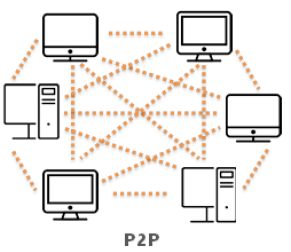
\includegraphics[width=0.4\textwidth]{./peer-to-peer}
\end{center}
